% ======================================
%             Chapter 2A.4
%           Active Transport
%        Created by Michael Tang
%             2025.02.23
% ======================================

\subsubsection{2A.4 Active Transport}
\paragraph{What is Active Transport?}
\begin{itemize}
    \item Active transport moves substances against their concentration gradient (from low to high concentration), requiring
    ATP (energy).
    \item This process is crucial for maintaining concentration gradients of ions and molecules within and outside the cell.
    \item Carrier proteins are used to move substances across the membrane.
\end{itemize}
\begin{figure}[H]
    \centering
    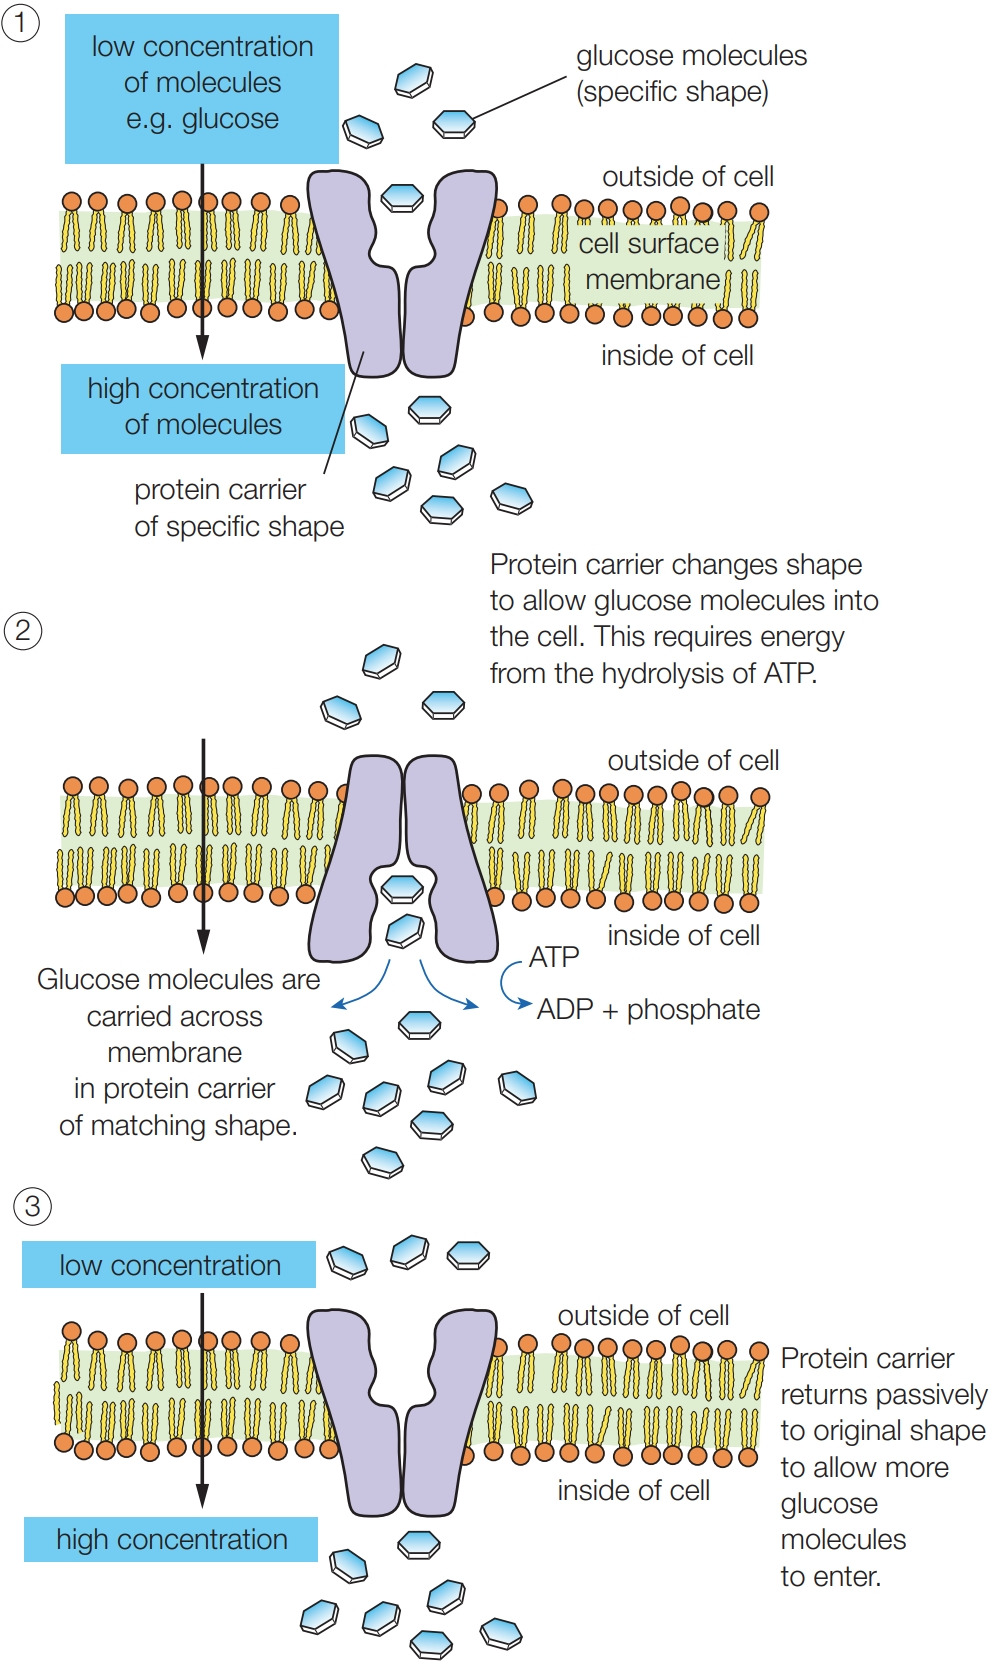
\includegraphics[scale=0.2]{Biology/2A/Images/2A-4-1.png}
    \caption{Using active transport, cells can move selected substances into or out of the cell, even when the concentration
    gradient is in the wrong direction.}
\end{figure}

\paragraph{How Active Transport Works}
\begin{itemize}
    \item Carrier proteins bind to the substance (e.g., glucose).
    \item ATP provides energy for the protein to change shape, allowing the molcule to be transported.
    \item Once the molecule is inside the cell, the carrier returns to its original shape.
\end{itemize}

\paragraph{Energy Source: ATP}
\begin{itemize}
    \item Active transport requires ATP to provide the energy needed for molecules to move against their concentration gradient.
    \item ATP hydrolysis (breaking down ATP into ADP + phosphate) releases the energy required to change the shape of the carrier
    protein.
\end{itemize}

\paragraph{Sodium-Potassium Pump}
A classic example of active transport is the sodium-potassium pump:
\begin{itemize}
    \item \textbf{Sodium ions (\ce{Na^+})} are pumped out of the cell.
    \item \textbf{Potassium ions (\ce{K^+})} are pumped into the cell.
    \item This process helps maintain the resting membrane potential in cells, expecially in nerve and muscle cells.
\end{itemize}

\paragraph{Endocytosis and Exocytosis}
\begin{itemize}
    \item \textbf{Endocytosis:} The process of taking materials into the cell by forming vesicles. This can be used for large
    molecules like bacteria (\underline{phagocytosis} 吞噬作用) or liquids (\underline{pinocytosis} 胞饮作用).
    \begin{itemize}
        \item \textbf{Phagocytosis:} The cell \underline{engulfs} (吞没) large particles such as bacteria.
        \begin{figure}[H]
            \centering
            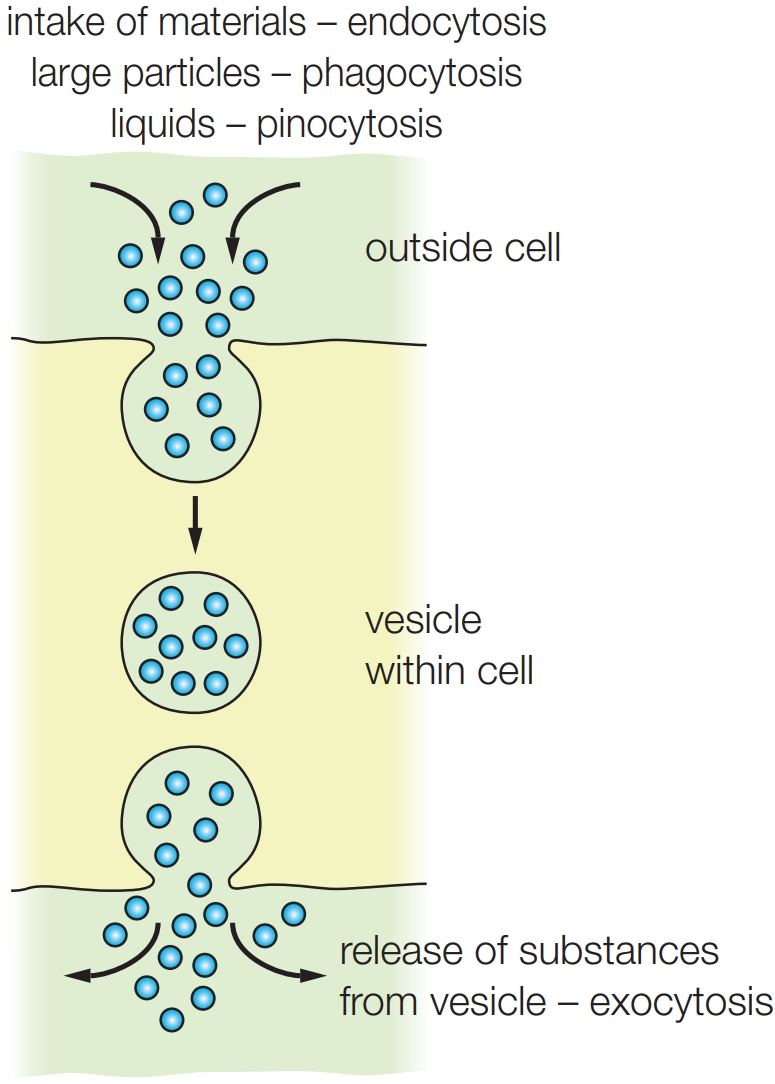
\includegraphics[scale=0.2]{Biology/2A/Images/2A-4-2.png}
            \caption{The properties of the cell membrane allow cells to take in large particles or release secretions.}
        \end{figure}
        \item \textbf{Pinocytosis:} The cell takes in liquids and small solutes.
        \begin{figure}[H]
            \centering
            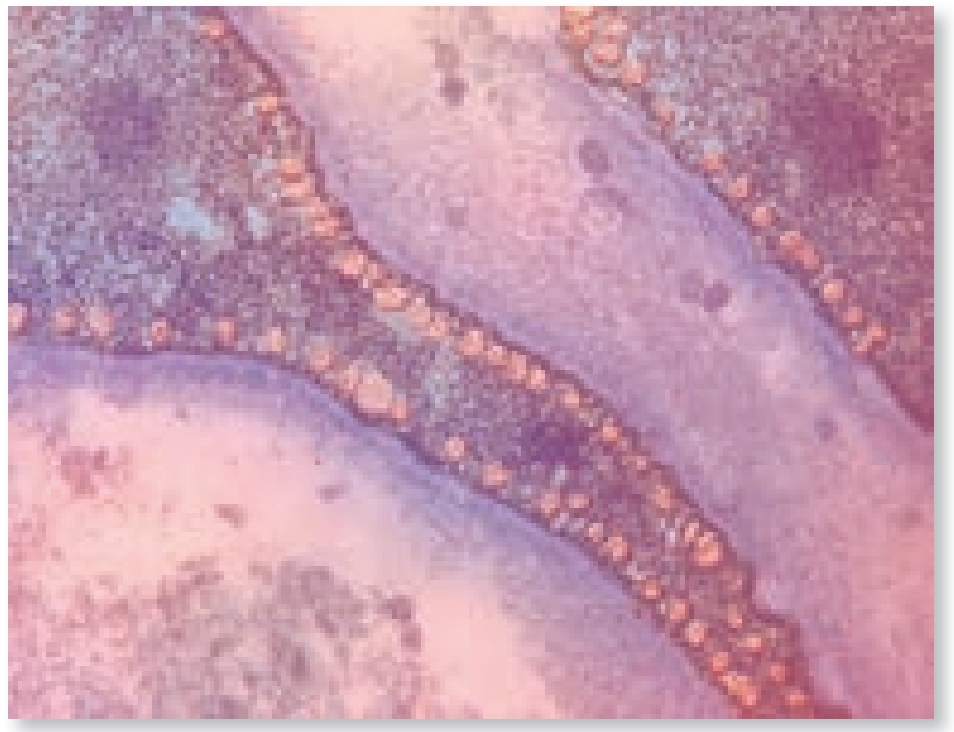
\includegraphics[scale=0.2]{Biology/2A/Images/2A-4-3.png}
            \caption{The mass of tiny vesicles along these cell membranes show pinocytosis.}
        \end{figure}
    \end{itemize}
\end{itemize}

\paragraph{The Fluid Mosaic Model of Membranes}
The processes of active transport, endocytosis, and exocytosis are facilitated by the fluid mosaic model of the cell membrane.
\begin{itemize}
    \item Carrier proteins and vesicles (formed from the membrane) play a central role in these processes.
    \item The flexible nature of the membrane allows for vesicle formation and fusion.
\end{itemize}

\paragraph{Exam Tips}
\begin{itemize}
    \item Always highlight that acive transport requires energy (ATP) and is against the concentration gradient.
    \item For endocytosis and exocytosis, focus on the vesicle formation and its fusion with the membrane.
    \item Explain ATP's role clearly in processes that need energy for molecular movement (e.g., active transport, vesicle
    fusion).
\end{itemize}